\section{Forts. Icke-linjära ekvationer}

\noindent Vi börjar med exemplet $e^x=10\cos(x) \Lrarr e^x-10\cos(x)$. Vi ska göra koden:
\par\bigskip

\begin{verbatim}
import numpy as np
import matplotlib.pyplot as plt

def bisection(func, a, b, tol):
    # sign_fa = np.sign(func(a))
    # sign_fb = np.sign(func(b))

    x = (a+b)/2
    itercounter = 0
    sign = np.sign(func(a)) == np.sign(func(b))

    assert(not sign)

    while((b-a)/2) > tol:
        
        itercounter += 1
        localSign = np.sign(func(x))

        if sign == localSign:
            a = x
        else:
            b = x

      x = (a+b)/2
    return x, itercounter
\end{verbatim}
\par\bigskip
\noindent Hitta en positiv lösning ($x>0$) till ekvationen med 8 korrekta decimaler.

\begin{itemize}
  \item Använd bisection
  \item Använd Newton-Raphson
\end{itemize}
\par\bigskip
\noindent Man börjar givetvis alltid med att skriva om på formen $f(x) = e^x-10\cos(x)$. Vi behöver också ett startintervall/startgissning, men hur ska man hitta det? Ett sätt är att fundera över hur funktionen ser ut. Ett annat sätt är att plotta funktionen (beror lite på det specifika fallet man undersöker). \par\noindent Vi ser att $f(0) = 1-10 = 9 <0$ och $f(\dfrac{\pi}{2}) = e^{\pi/2}-0 > 0$.\par\noindent. Vi testar att plotta vår funktion:

\begin{verbatim}
func = lambda x: np.exp(x)-10*np.cos(x) 
\end{verbatim}
\par\bigskip
\noindent Här ser vi en rot mellan 1 och 1.5:

\begin{center}
  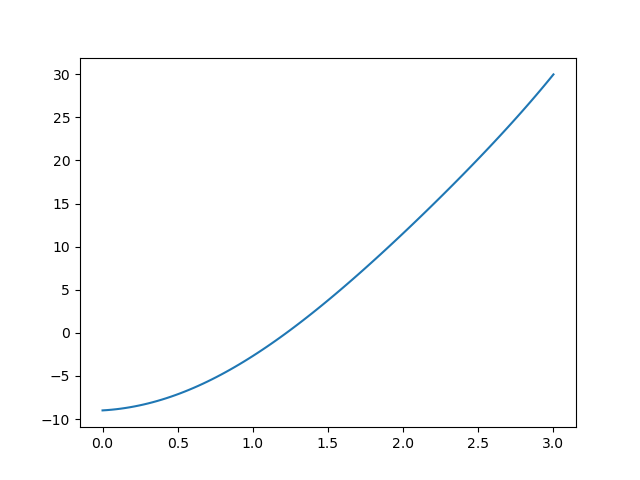
\includegraphics{figures/Figure_1.png}
\end{center}

\pagebreak
\noindent Kör vi koden får vi att den konvergerar mot $\approx$ 1.2 med 26 iterationer. Implementerar vi Newtons metod och använder startvärde 1.25 får vi konvergens med inget mindre än 4 iterationer! Givetvis måste vi dock räkna derivator. 
\par\bigskip
\noindent \textit{Slutsats:} Newton är mycket snabbare.\par\noindent Frågan är varför? Kan det bero på likformig kontinuitet eller strikt monoton?
\par\bigskip

\subsection{Konvergenshastighet}\hfill\\

\noindent Låt $x_*$ vara vår exakta lösning och vi antar att vi har en iterativ metod som generar en talföljd $x_1, x_2, \cdots$. Antag även att vi har konvergens, dvs $\lim_{k\to\infty}x_k = x_*$.
\par\bigskip
\begin{theo}[Konvergensordning]{thm:orderofconv}
  En metod har \textit{konvergensordning} $r$ om $\lim_{k\to\infty}\dfrac{\left|x_*-x_{k+1}\right|}{\left|x_*-x_k\right|^r} = C$ där $C$ (konstant) kallas för \textit{asymptotisk felkonstant} 
\end{theo}
\par\bigskip
\noindent Notera att ju större $r$ är, desto snabbare konvergerar den. Om:

\begin{itemize}
  \item $r=1, C<1$ har vi \textit{linjär konvergens}
  \item $r=2$ har vi \textit{kvadratisk konvergens}
  \item $r>1$ har vi \textit{superlinjär konvergens} (Busigt att använda $r>1$)
\end{itemize}
\par\bigskip

\subsection{Konvergens i bisektionsmetoden}\hfill\\

\noindent Felet halveras i varje steg. Vi kommer ihåg att vi har $\left|x_*-x_k\right|\leq \dfrac{B-A}{2^k}$ där $[A,B]$ är startintervallet. Det nya felet kommer då vara $\dfrac{1}{2}$ gamla felet, därför har vi $r=1$ och $C=\dfrac{1}{2}$ det vill säga linjär konvergens.
\par\bigskip

\subsection{Konvergens i Newton-Raphson}\hfill\\

\noindent Påminner oss om metoden: $x_{k+1} = x_k -\dfrac{f(x_k)}{f^{\prime}(x_k)}$ . Vi Taylorutvecklar kring $x_k$ med steget $(x_*-x_k)$. sedan har vi $\underbrace{f(x_k+(x_*-x_k))}_{\text{$f(x_*)=0$}} = f(x_k)+(x_*-x_k)f^{\prime}(x_k)+(x_*-x_k)^2f^{\prime\prime}(\xi)\cdot\dfrac{1}{2}$ 













